\documentclass[11pt,a4paper]{article}
\usepackage[utf8]{inputenc}
\usepackage[T1]{fontenc}
\usepackage{lmodern}
\usepackage[brazil]{babel}
\usepackage[margin=2cm]{geometry}
\usepackage{microtype}
\usepackage{booktabs,multirow,array}
\usepackage{graphicx}
\usepackage{float}
\usepackage[section]{placeins}
\usepackage[font=small,labelfont=bf]{caption}
\usepackage{enumitem}
\usepackage[dvipsnames]{xcolor}
\usepackage{tcolorbox}
\usepackage{fancyhdr}
\usepackage[hidelinks]{hyperref}

\graphicspath{{../../v3_reeval/figures/}}
\setlist{itemsep=2pt,topsep=3pt}
\newtcolorbox{achado}[1]{colback=blue!3,colframe=blue!50!black,title={#1},fonttitle=\bfseries,boxrule=0.6pt,arc=1mm}
\newtcolorbox{alerta}[1]{colback=orange!5,colframe=orange!70!black,title={#1},fonttitle=\bfseries,boxrule=0.6pt,arc=1mm}
\newcommand{\system}{\textsc{Norma}}

\pagestyle{fancy}
\fancyhf{}
\lhead{\small Norma --- rodada oficial v3 (seis datasets)}
\rhead{\small 19 de outubro de 2026}
\cfoot{\small\thepage}

\title{\textbf{Norma: rodada oficial v3 (E1--E3) com seis datasets}\\[2pt]
\large Correções, novas implementações, resultados e recomendações para a nova versão do artigo (VLDB)}
\author{Junio Freitas}
\date{15 de outubro de 2026; revisado em 19 de outubro de 2026}

\begin{document}
\maketitle
\thispagestyle{fancy}

\section*{Resumo}

Reexecutamos os experimentos da Seção~6 do artigo do \system\ (E1 classificação; E2 mapeamento; E3 fim a fim,
\textbf{sem} o modo \emph{document-level}) depois de um ciclo de correções e melhorias no sistema, no ground truth
(GT) e na avaliação. A rodada cobre os \textbf{quatro datasets do artigo} (Hospital, Restaurant, SISU, Tax) e os
\textbf{dois datasets HMDA} (HMDAZ e HMDA Checks), com \textbf{seis LLMs} via OpenRouter: GPT-6 Luna,
DeepSeek-V4-Flash, Mistral Large 4, Qwen3.8-2.4T-A95B, GPT-6 Sol e Claude Sonnet 5.5. Cada configuração foi
executada \textbf{uma vez}. Foram 138 jobs (36 do E1, 72 do E2, 12 do E3, mais 18 do modelo substituído), todos
concluídos; o custo cobrado foi de US\$~82,94. Os números deste relatório já incorporam a correção da
semântica das DCs de duas tuplas na tradução para SQL e a reavaliação das saídas gravadas, sem novas chamadas a
LLM (Seção~\ref{sec:pares}).

\begin{itemize}
  \item \textbf{E1:} só três configurações atingem recall $\geq$ 0,90 em todos os datasets. A escolhida é
        \emph{Qwen3.8-2.4T-A95B + Examples} (F$_1$ médio 0,69), a mesma família e o mesmo prompt do artigo. O gargalo
        de recall é o HMDAZ (16 das 24 configurações acertam só 4 das 9 regras). Na HMDA Checks, sem contexto de
        tabela todos os modelos rotulam quase tudo como regra (F$_1$ 0,74 = classificador trivial).
  \item \textbf{E2:} nos quatro datasets do artigo, o Multi-Step volta a superar o Single-Prompt (CE 0,80 contra
        0,75; AV 0,89 contra 0,55) e os melhores modelos novos superam o GPT-5 do artigo (Sonnet 0,84/0,97; Sol e
        Mistral 0,81/0,99; GPT-5 0,78/0,95). Nos HMDA, a extração por equivalência recupera boa parte do que a
        extração exata perde, e a aparente vantagem do Single-Prompt na AV da HMDA Checks é um artefato de
        concentração das violações.
  \item \textbf{E3:} \system\ extrai as regras do GT em todos os datasets (CE 1,00 em Hospital e Tax; 0,58--0,59
        na HMDA Checks). A AV agregada, porém, fica baixa no Tax (0,15) e no SISU com C+MS (0,11) por causa de
        \emph{uma} DC ampla em cada caso; o classificador reduz o custo do pipeline de 1,6 a 5 vezes.
  \item \textbf{Avaliação:} em 4 dos 6 datasets uma única regra concentra de 78\% a 99\% das tuplas violadoras.
        Recomendamos reportar, ao lado da AV, o F$_1$ médio por regra e a equivalência por execução.
  \item \textbf{Correção na tradução para SQL:} as DCs de duas tuplas usavam \texttt{t1.tid < t2.tid}, o que perde
        violações de DCs assimétricas. Corrigido para \texttt{t1.tid <> t2.tid}; só o SISU muda (violações do GT de
        487 para 533) e nenhuma conclusão se inverte.
\end{itemize}

\section{Escopo, protocolo e execução}

\subsection{Datasets}

\begin{table}[H]
\centering\small\setlength{\tabcolsep}{4.5pt}
\begin{tabular}{lrrrrrrr}
\toprule
Dataset & Linhas usadas & Cols & Sent. & Regras & Tuplas viol. & Maior regra & Regras sem viol.\\
\midrule
Hospital & 1.006 & 17 & 109 & 15 & 834 & 0,96 & 0\\
Restaurant & 127.692 & 21 & 33 & 7 & 52.311 & 0,99 & 0\\
SISU & 101.717 & 56 & 42 & 17 & 533 & 0,60 & 0\\
Tax & 99.906 & 15 & 126 & 6 & 468 & 0,78 & 0\\
HMDAZ & 1.000.000 (de 15,1M) & 135 & 17 & 9 & 209 & 0,54 & 1\\
HMDA Checks & 1.000.000 (de 4,8M) & 81 & 158 & 92 & 986.491 & 0,99 & 68\\
\bottomrule
\end{tabular}
\caption{Datasets da rodada. ``Regras'' conta as sentenças com DC não nula no GT; ``Maior regra'' é a fração das
tuplas violadoras marcadas pela maior regra do GT (concentração); ``Regras sem viol.'' conta regras do GT sem
nenhuma violação no recorte.}
\end{table}

\noindent Os GTs dos quatro datasets do artigo não mudaram (as violações batem com a Tabela~2 do artigo). Os GTs
dos HMDA foram revistos contra os documentos-fonte (Seção~\ref{sec:mudancas}).

\subsection{Modelos e substituições}

\begin{table}[H]
\centering\footnotesize\setlength{\tabcolsep}{4.5pt}
\begin{tabular}{llrrr}
\toprule
Modelo & Slug (OpenRouter) & US\$/M tok. (entr./saída) & Chamadas & Custo (US\$)\\
\midrule
GPT-6 Luna & \texttt{openai/gpt-6-luna} & 0,10 / 0,50 & 854 & 0,77\\
DeepSeek-V4-Flash & \texttt{deepseek/deepseek-v4-flash} & 0,09 / 0,18 & 871 & 0,74\\
Mistral Large 4 & \texttt{mistralai/mistral-large-4-0} & 0,68 / 2,09 & 856 & 8,93\\
Qwen3.8-2.4T-A95B & \texttt{qwen/qwen3.8-2.4t-a95b} & 2,00 / 6,00 & 913 & 17,32\\
GPT-6 Sol & \texttt{openai/gpt-6-sol} & 2,00 / 10,00 & 3.142 & 36,02\\
Claude Sonnet 5.5 & \texttt{anthropic/claude-sonnet-5.5} & 2,00 / 10,00 & 859 & 17,62\\
\midrule
MiniMax-M3 (substituído) & \texttt{minimax/minimax-m3} & 0,30 / 1,20 & 912 & 1,54\\
\midrule
\multicolumn{3}{l}{Total} & 8.407 & 82,94\\
\bottomrule
\end{tabular}
\caption{LLMs da rodada. O GPT-6 Sol tem mais chamadas porque também é o mapper do E3 (inclui a execução do E3
interrompida por falta de crédito). Custos medidos por requisição; o harness contabilizou US\$~85,82, porque
inclui reservas de requisições abortadas.}
\end{table}

A lista original tinha o \textbf{Kimi K2.6}. No \emph{health check}, sob decodificação estrita por
\emph{JSON Schema}, ele emitia espaços em branco até o limite de tokens em dois passos do Multi-Step, em todos os
provedores testados (6 de 6 falhas no roteamento padrão; 1 de 6 acertos no provedor bf16). Por decisão dos
autores, foi substituído pelo \textbf{MiniMax-M3}, que passou no health check. No E2, porém, o MiniMax devolveu
\texttt{\{"results":[]\}} para 107 das 156 sentenças do Single-Prompt v2, embora completasse o Multi-Step sem
falhas; testado isoladamente, com prompt curto, respondia corretamente. Também por decisão dos autores, ele foi
substituído pelo \textbf{Mistral Large 4}, o único entre quatro candidatos (MiMo-V2.6-Pro, Nemotron~3 Ultra,
Seed~2.1 Turbo) que passou em todos os testes do health check \emph{estendido}, que agora inclui o schema do
Single-Prompt v2. Os resultados do MiniMax estão em \texttt{results/v3/superseded/}.

\subsection{Protocolo}

\begin{itemize}
  \item \textbf{E1:} 4 prompts $\times$ 6 modelos $\times$ 6 datasets, lotes de 10 sentenças; seleção por
        recall $\geq$ 0,90 em todos os datasets e maior F$_1$ médio.
  \item \textbf{E2:} Single-Prompt e Multi-Step (2 iterações de refinamento) só nas sentenças do GT. O
        Single-Prompt usa a versão melhorada (prompt \texttt{with\_examples\_v2}, lotes de 3, campo
        \texttt{violated\_when}, seleção semântica de colunas com \emph{embeddings} \texttt{text-embedding-3-large}
        e contexto de colunas). Seleção do mapper do E3: melhor Multi-Step em CE e AV.
  \item \textbf{E3:} C+MS e Multi-Step sobre todas as sentenças, com os componentes escolhidos.
  \item \textbf{Comum:} espaço de predicados v2 (sob demanda) em todos os datasets; saída estruturada estrita;
        no máximo 32.768 tokens de saída por chamada; 1 execução por configuração; DuckDB com limite de
        memória e tempo; primeiras 1M linhas dos HMDA.
\end{itemize}

\subsection{Ocorrências durante a execução}

Todas registradas em \texttt{results/v3/telemetry/20261013\_215731\_662134/CHANGES.md}:
\begin{enumerate}
  \item Troca Kimi K2.6 $\rightarrow$ MiniMax-M3 antes de qualquer job do Kimi (orquestrador parado e retomado).
  \item 13 erros transitórios de conexão, todos recuperados por novas tentativas com \emph{backoff}.
  \item Parada por falta de crédito no OpenRouter (HTTP 402) durante o E3. O job interrompido (Multi-Step na
        HMDA Checks) foi refeito do zero e o resultado parcial movido para \texttt{superseded}. O motivo de parada
        foi limpo à mão no \texttt{summary.json} para permitir a retomada.
  \item Troca MiniMax-M3 $\rightarrow$ Mistral Large 4 e nova aplicação dos critérios de seleção do E3
        (componentes inalterados).
\end{enumerate}

\section{O que mudou no \system\ desde a submissão}
\label{sec:mudancas}

\subsection{Correções}
\begin{enumerate}
  \item \textbf{Método genérico.} O prompt do Multi-Step tinha exemplos que reproduziam sentenças do GT do HMDAZ e
        paráfrases do GT do Restaurant (vazamento de teste), e o código tinha quatro reparos fixos de HMDA
        (código $\rightarrow$ \texttt{*\_name}, \texttt{rate\_spread}, pontos percentuais e ``exceed''). Os
        exemplos foram trocados por exemplos neutros e os reparos removidos; não restam referências fixas a
        datasets no código do método.
  \item \textbf{Robustez dos mappers.} Validação com tipos (por exemplo, \texttt{rate\_spread != 'NA'} é
        rejeitada); reparo de nós AND/OR unários ou vazios antes da validação; o Single-Prompt devolve ao modelo,
        uma vez, as regras inválidas com a mensagem de erro; o Multi-Step normaliza nomes de colunas e
        repergunta quando o JSON vem malformado.
  \item \textbf{Falhas contadas.} Erros de SQL das regras previstas passam a ser contados, em vez de virarem
        ``zero violações'' em silêncio; o \emph{predicate Jaccard} passa a ser calculado sobre os
        predicados-folha.
  \item \textbf{GT dos HMDA.} \emph{HMDAZ}: sentenças literais da Regulation~Z de 2018, gatilhos HOEPA com as
        condições de cobertura, novas regras (\emph{balloon}, amortização negativa, multa de pré-pagamento) e
        remoção da §1026.43(g)(1); 17 entradas, 9 com regra. \emph{HMDA Checks}: realinhada ao guia de edições de
        2014 do FFIEC, a mesma versão dos dados, com uma entrada por edição e as edições não verificáveis por
        registro como \texttt{null}; 158 entradas, 92 com regra (positivos no E1 caíram de 93\% para 58\%).
\end{enumerate}

\subsection{Novas implementações}
\begin{enumerate}
  \item \textbf{Espaço de predicados v2 (sob demanda).} O arquivo do dataset guarda só o esquema: tipo,
        operadores, operadores aritméticos, valores de domínio e uma descrição de cada coluna, escrita uma vez
        por LLM a partir de um perfil determinístico dos dados. Os predicados são gerados em tempo de execução
        só para as colunas selecionadas. Invariante testado: para os mesmos dados e opções, a geração é igual
        ao espaço v1 restrito às colunas. Nos datasets do artigo, a v2 reproduz a v1 exatamente (318, 414,
        5.112 e 482 templates); no HMDAZ, evita materializar 590 mil templates.
  \item \textbf{Glossário oficial.} As definições do FFIEC foram incorporadas às descrições de 36 colunas do
        HMDAZ (e das colunas de rótulo correspondentes).
  \item \textbf{Single-Prompt v2.} Prompt \texttt{with\_examples\_v2} com contexto de colunas, semântica de
        violação e campo \texttt{violated\_when}; seleção de colunas léxica, semântica ou híbrida. Na
        validação com GPT-6 Luna, a CE média em cinco datasets passou de 0,56 para 0,64.
  \item \textbf{Avaliação.}
        (i)~\emph{Extração por equivalência lógica} (CE$_\equiv$): forma normal disjuntiva (IN$\leftrightarrow$OR,
        ordem dos operandos, distributiva, absorção) e unificação de literais código/rótulo apenas quando os
        dados confirmam que selecionam as mesmas linhas; os pares são descobertos nos dados.
        (ii)~\emph{Equivalência por execução}: fração das regras do GT (com $\geq 1$ violação) cuja regra prevista
        marca exatamente as mesmas linhas. (iii)~\emph{F$_1$ médio por regra}. (iv)~\emph{Concentração} da AV
        (\texttt{max\_gold\_rule\_violation\_share}) e regras do GT sem violação.
  \item \textbf{Execução.} Health check estendido (classificador, os dois schemas do Single-Prompt e os cinco
        schemas do Multi-Step); opção \texttt{json\_object\_models} para modelos com decodificação estrita
        instável (implementada para o Kimi K2.6 e não usada na rodada final); controle de orçamento,
        paralelismo com exclusividade por modelo e limite de memória.
\end{enumerate}

\section{Hipóteses}

\begin{enumerate}[label=H\arabic*.]
  \item O espaço sob demanda com descrições de colunas melhora o mapeamento em esquemas largos sem alterar o
        resultado nos datasets do artigo.
  \item Parte do erro de extração nos HMDA é de forma, não de conteúdo (equivalência lógica, código
        $\leftrightarrow$ rótulo); uma métrica de equivalência deve recuperá-la.
  \item A AV agregada é dominada pela regra mais violada; métricas por regra mudam a leitura dos resultados.
  \item O Multi-Step continua superior ao Single-Prompt mesmo depois das melhorias no Single-Prompt.
  \item O classificador continua útil no pipeline fim a fim, agora também em datasets grandes.
\end{enumerate}

\section{E1 --- Classificação de sentenças}

\begin{figure}[H]
\centering
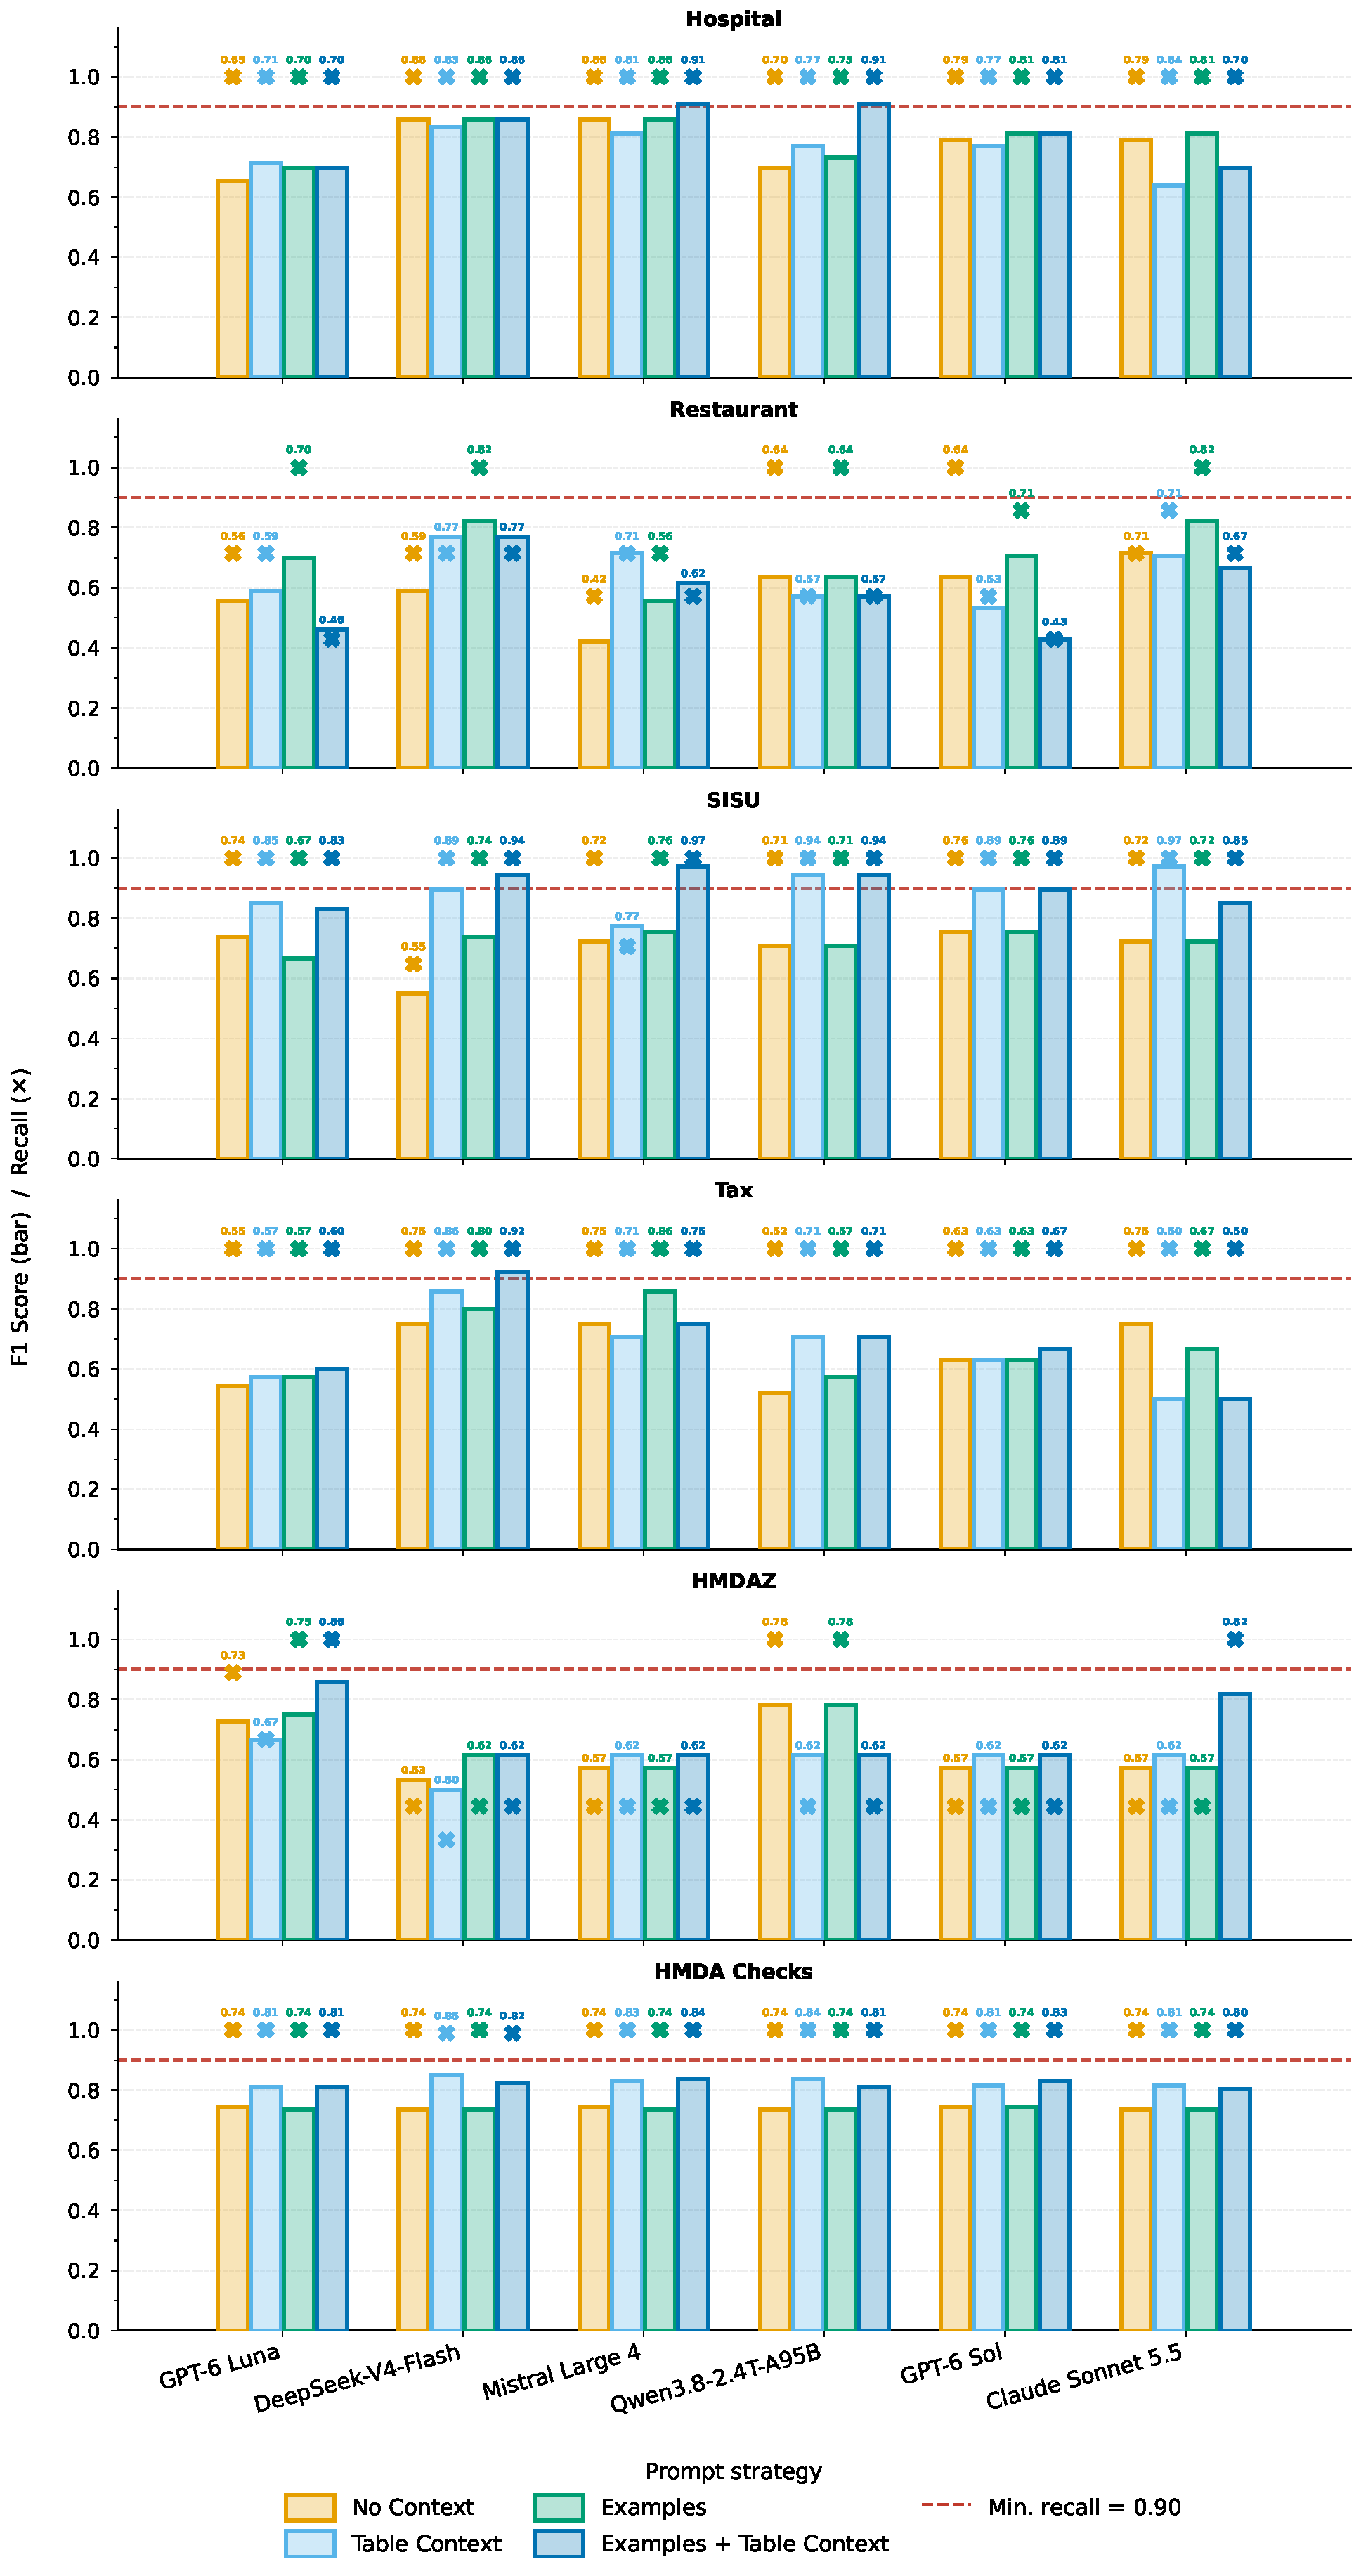
\includegraphics[width=0.78\textwidth]{v3_fig6_classifiers.pdf}
\caption{F$_1$ (barras) e recall (\textsf{x}) por modelo e prompt (formato da Figura~6 do artigo).}
\end{figure}

\begin{table}[H]
\centering\small
\begin{tabular}{lcccc}
\toprule
Modelo & No Context & Table Context & Examples & Examples + Table\\
\midrule
GPT-6 Luna & 0,66 (0,71) & 0,70 (0,67) & 0,69 (\textbf{1,00}) & 0,71 (0,43)\\
DeepSeek-V4-Flash & 0,67 (0,44) & 0,78 (0,33) & 0,76 (0,44) & 0,82 (0,44)\\
Mistral Large 4 & 0,68 (0,44) & 0,74 (0,44) & 0,72 (0,44) & 0,78 (0,44)\\
Qwen3.8-2.4T-A95B & 0,68 (\textbf{1,00}) & 0,74 (0,44) & \textbf{0,69 (1,00)} & 0,76 (0,44)\\
GPT-6 Sol & 0,69 (0,44) & 0,71 (0,44) & 0,70 (0,44) & 0,71 (0,43)\\
Claude Sonnet 5.5 & 0,71 (0,44) & 0,71 (0,44) & 0,72 (0,44) & 0,72 (0,71)\\
\bottomrule
\end{tabular}
\caption{F$_1$ médio nos seis datasets e, entre parênteses, o menor recall. Só as configurações com menor recall
1,00 são elegíveis; em negrito, a escolhida.}
\end{table}

\begin{achado}{Achados do E1}
\begin{itemize}
  \item \textbf{Critério do artigo aplicado:} elegíveis Qwen + Examples (0,694), Luna + Examples (0,687) e
        Qwen + No Context (0,680). A melhor média sem o critério (DeepSeek + Examples + Table, 0,82) perde mais
        da metade das regras do HMDAZ.
  \item \textbf{HMDAZ limita o recall:} as definições da Regulation~Z (``um empréstimo é \emph{high-cost} se\dots'')
        soam como escopo, mas implicam condições verificáveis. 16 das 24 configurações acertam só 4 das 9.
  \item \textbf{HMDA Checks e o contexto de tabela:} sem contexto, F$_1$ = 0,74, o mesmo do classificador
        ``tudo positivo''. Com contexto de tabela, 0,80--0,85. As edições não verificáveis por registro só se
        distinguem pela estrutura do registro.
  \item \textbf{Comparação com o artigo (4 datasets):} F$_1$ médio de todas as configurações subiu de 0,69 para
        0,72, mas a melhor elegível caiu (0,66 contra 0,85 do Qwen3-32B): os modelos novos aceitam mais
        sentenças, mantendo o recall e perdendo precisão (Tax, Restaurant).
\end{itemize}
\end{achado}

\section{E2 --- Mapeamento}

\begin{figure}[H]
\centering
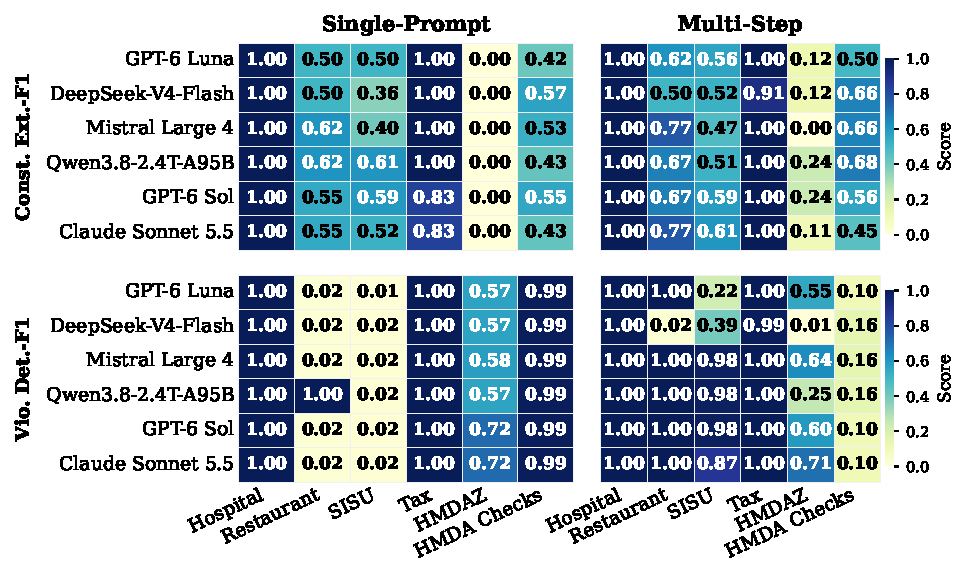
\includegraphics[width=0.9\textwidth]{v3_fig7_mapping.pdf}
\caption{CE (extração exata) e AV (violação agregada) por modelo e mapper, só nas sentenças do GT (formato da
Figura~7 do artigo).}
\end{figure}

\begin{table}[H]
\centering\small\setlength{\tabcolsep}{4pt}
\begin{tabular}{llrrrrrr}
\toprule
\textbf{Mapper} & \textbf{Model} & CE & CE$_{\equiv}$ & AV & Rule-F$_1$ & Exec. & Fail. \\
\midrule
\multirow{6}{*}{Single-Prompt} & GPT-6 Luna & 0.57 & 0.69 & 0.60 & 0.78 & 0.75 & 0 \\
 & DeepSeek-V4-Flash & 0.57 & 0.66 & 0.60 & 0.74 & 0.70 & 3 \\
 & Mistral Large 4 & 0.59 & 0.66 & 0.60 & 0.73 & 0.71 & 0 \\
 & Qwen3.8-2.4T-A95B & 0.61 & 0.70 & 0.76 & \textbf{0.86} & \textbf{0.83} & 0 \\
 & GPT-6 Sol & 0.59 & 0.67 & 0.62 & 0.76 & 0.72 & 0 \\
 & Claude Sonnet 5.5 & 0.55 & 0.64 & 0.62 & 0.76 & 0.70 & 0 \\
\midrule
\multirow{6}{*}{Multi-Step} & GPT-6 Luna & 0.63 & 0.68 & 0.65 & 0.75 & 0.73 & 0 \\
 & DeepSeek-V4-Flash & 0.62 & 0.64 & 0.43 & 0.68 & 0.67 & 0 \\
 & Mistral Large 4 & 0.65 & 0.72 & \textbf{0.80} & 0.81 & 0.80 & 0 \\
 & Qwen3.8-2.4T-A95B & \textbf{0.68} & 0.70 & 0.73 & 0.76 & 0.74 & 0 \\
 & GPT-6 Sol & 0.67 & 0.71 & 0.78 & 0.80 & 0.79 & 0 \\
 & Claude Sonnet 5.5 & 0.66 & \textbf{0.73} & 0.78 & 0.84 & 0.81 & 0 \\
\bottomrule
\end{tabular}

\caption{Médias nos seis datasets. CE$_\equiv$: extração por equivalência; Rule-F$_1$: F$_1$ médio por regra;
Exec.: equivalência por execução; Fail.: sentenças sem saída válida do modelo.}
\end{table}

\begin{table}[H]
\centering\small
\begin{tabular}{lcccc}
\toprule
 & \multicolumn{2}{c}{4 datasets do artigo} & \multicolumn{2}{c}{HMDAZ + HMDA Checks}\\
\cmidrule(lr){2-3}\cmidrule(lr){4-5}
Métrica & Single-Prompt & Multi-Step & Single-Prompt & Multi-Step\\
\midrule
CE & 0,75 & \textbf{0,80} & 0,24 & \textbf{0,36}\\
CE$_\equiv$ & 0,75 & \textbf{0,80} & \textbf{0,51} & 0,49\\
AV & 0,55 & \textbf{0,89} & \textbf{0,81} & 0,29\\
Rule-F$_1$ & 0,78 & \textbf{0,84} & \textbf{0,74} & 0,64\\
Exec. & 0,77 & \textbf{0,83} & \textbf{0,67} & 0,61\\
\bottomrule
\end{tabular}
\caption{Médias sobre os seis modelos por grupo de datasets.}
\end{table}

\begin{table}[H]
\centering\scriptsize\setlength{\tabcolsep}{3pt}
\begin{tabular}{llcccccccc}
\toprule
 & & \multicolumn{2}{c}{Restaurant} & \multicolumn{2}{c}{Tax} & \multicolumn{2}{c}{Hospital} & \multicolumn{2}{c}{HMDA Checks} \\
\cmidrule(lr){3-4}\cmidrule(lr){5-6}\cmidrule(lr){7-8}\cmidrule(lr){9-10}
Mapper & Model & full & w/o & full & w/o & full & w/o & full & w/o \\
\midrule
\multirow{6}{*}{Single-Prompt} & GPT-6 Luna & 0.02 & 1.00 & 1.00 & 1.00 & 1.00 & 1.00 & 0.99 & 0.77 \\
 & DeepSeek-V4-Flash & 0.02 & 1.00 & 1.00 & 1.00 & 1.00 & 1.00 & 0.99 & 0.18 \\
 & Mistral Large 4 & 0.02 & 1.00 & 1.00 & 1.00 & 1.00 & 1.00 & 0.99 & 0.74 \\
 & Qwen3.8-2.4T-A95B & 1.00 & 1.00 & 1.00 & 1.00 & 1.00 & 1.00 & 0.99 & 1.00 \\
 & GPT-6 Sol & 0.02 & 1.00 & 1.00 & 1.00 & 1.00 & 1.00 & 0.99 & 0.18 \\
 & Claude Sonnet 5.5 & 0.02 & 1.00 & 1.00 & 1.00 & 1.00 & 1.00 & 0.99 & 1.00 \\
\midrule
\multirow{6}{*}{Multi-Step} & GPT-6 Luna & 1.00 & 1.00 & 1.00 & 1.00 & 1.00 & 1.00 & 0.10 & 1.00 \\
 & DeepSeek-V4-Flash & 0.02 & 1.00 & 0.99 & 0.96 & 1.00 & 1.00 & 0.16 & 0.77 \\
 & Mistral Large 4 & 1.00 & 1.00 & 1.00 & 1.00 & 1.00 & 1.00 & 0.16 & 0.77 \\
 & Qwen3.8-2.4T-A95B & 1.00 & 1.00 & 1.00 & 1.00 & 1.00 & 1.00 & 0.16 & 0.77 \\
 & GPT-6 Sol & 1.00 & 1.00 & 1.00 & 1.00 & 1.00 & 1.00 & 0.10 & 1.00 \\
 & Claude Sonnet 5.5 & 1.00 & 1.00 & 1.00 & 1.00 & 1.00 & 1.00 & 0.10 & 1.00 \\
\bottomrule
\end{tabular}
\caption{Sensibilidade da AV do E2 à(s) regra(s) dominante(s): \emph{full} = GT completo; \emph{w/o} = sem a regra que marca $\geq$ 75\% das tuplas violadoras (Restaurant 99\%, Tax 78\%, Hospital 96\%) ou, na HMDA Checks, sem as edições de data S270 e Q022. SISU e HMDAZ não têm regra dominante.}
\end{table}


\begin{achado}{Achados do E2}
\begin{itemize}
  \item \textbf{H4 confirmada nos datasets do artigo.} Multi-Step supera o Single-Prompt melhorado em todas as
        métricas. Os melhores modelos superam o GPT-5 do artigo: Sonnet 0,84/0,97; Sol e Mistral 0,81/0,99.
  \item \textbf{Onde o Single-Prompt perde violações.} \emph{Restaurant:} cinco dos seis modelos devolvem
        \texttt{null} para ``pelo menos uma inspeção por ano'', que concentra 99\% das violações (recall
        0,01); sem essa regra, todos chegam a 1,00. \emph{SISU:} o Single-Prompt identifica o estudante pela
        inscrição do ENEM em vez do CPF nas regras entre duas tuplas e marca cerca de 51 mil tuplas contra 533
        (precisão $<$ 0,01).
  \item \textbf{H2 confirmada.} A CE$_\equiv$ praticamente não muda os datasets do artigo, mas nos HMDA eleva a
        CE de 0,24 para 0,51 (Single-Prompt) e de 0,36 para 0,49 (Multi-Step).
  \item \textbf{H3 confirmada (HMDA Checks).} O Single-Prompt marca AV 0,99 e o Multi-Step 0,10--0,16. Duas edições
        de data (S270, Q022) marcam 99\% das tuplas violadoras, que cobrem 98,6\% das linhas: uma DC que marca
        \emph{todas} as tuplas já obtém 0,99. O Multi-Step devolve \texttt{null} para as duas; a maioria das DCs do
        Single-Prompt marca todas as linhas (por exemplo, \texttt{action\_taken\_date / 10000 !=
        activity\_year}, sempre verdadeira em divisão real). Sem essas duas edições, a ordem se inverte (tabela
        de sensibilidade acima).
  \item \textbf{H1 (espaço sob demanda).} Não foi testada diretamente nesta rodada, que usou só a v2. Nos datasets do
        artigo, o invariante garante o mesmo vocabulário da v1. No HMDAZ, a evidência vem da validação anterior
        com GPT-6 Luna: a AV do Multi-Step passou de 0,18 (v1) para 0,68 (v2). Para afirmar isso no artigo, seria
        preciso uma ablação v1 $\times$ v2 com os modelos finais.
  \item \textbf{Escolha do mapper do E3.} Nenhum modelo lidera em CE e AV (Qwen CE 0,68; Mistral AV 0,80). Pela
        média das duas: Sol 0,727, Mistral 0,722, Sonnet 0,718, Qwen 0,707. Escolhido o GPT-6 Sol; com uma
        execução por configuração, é um empate técnico entre os quatro.
\end{itemize}
\end{achado}

\section{E3 --- Fim a fim}

\begin{table}[H]
\centering\footnotesize\setlength{\tabcolsep}{3.5pt}
\resizebox{\textwidth}{!}{\begin{tabular}{llccccccccc}
\toprule
\textbf{Family} & \textbf{Method} & \multicolumn{3}{c}{Constr. Classification} & \multicolumn{3}{c}{Constr. Extraction} & \multicolumn{3}{c}{Viol. Discovery} \\
\cmidrule(lr){3-5}  \cmidrule(lr){6-8}  \cmidrule(lr){9-11}
 &  & P & R & F$_1$ & P & R & F$_1$ & P & R & F$_1$ \\
\midrule
\addlinespace[2pt]
\multicolumn{11}{c}{\textbf{Hospital}} \\
\addlinespace[1pt]
\multirow{2}{*}{\system} & ~~C+MS & 0.83 & 1.00 & \textbf{0.91} & 1.00 & 1.00 & \textbf{1.00} & 1.00 & 1.00 & \textbf{1.00} \\
 & ~~Multi-Step & 0.71 & 1.00 & 0.83 & 1.00 & 1.00 & \textbf{1.00} & 1.00 & 1.00 & \textbf{1.00} \\
\cmidrule(l){2-11}
\multirow{1}{*}{Profiling} & ~~DC Discovery & n/a & n/a & n/a & 0.00 & 0.00 & 0.00 & 0.83 & 1.00 & 0.91 \\
\cmidrule(l){2-11}
\multirow{1}{*}{Text2SQL} & ~~XiYan-SQL & 0.50 & 1.00 & 0.67 & 0.60 & 1.00 & 0.75 & 0.83 & 1.00 & 0.91 \\
\midrule
\addlinespace[2pt]
\multicolumn{11}{c}{\textbf{Restaurant}} \\
\addlinespace[1pt]
\multirow{2}{*}{\system} & ~~C+MS & 1.00 & 0.71 & \textbf{0.83} & 0.80 & 0.57 & \textbf{0.67} & 1.00 & 1.00 & \textbf{1.00} \\
 & ~~Multi-Step & 1.00 & 0.71 & \textbf{0.83} & 0.80 & 0.57 & \textbf{0.67} & 1.00 & 1.00 & \textbf{1.00} \\
\cmidrule(l){2-11}
\multirow{1}{*}{Profiling} & ~~DC Discovery & n/a & n/a & n/a & 0.00 & 0.00 & 0.00 & 0.77 & 0.87 & 0.82 \\
\cmidrule(l){2-11}
\multirow{1}{*}{Text2SQL} & ~~XiYan-SQL & 0.86 & 0.75 & 0.80 & 0.17 & 0.12 & 0.14 & 0.45 & 0.64 & 0.52 \\
\midrule
\addlinespace[2pt]
\multicolumn{11}{c}{\textbf{SISU}} \\
\addlinespace[1pt]
\multirow{2}{*}{\system} & ~~C+MS & 0.84 & 0.94 & \textbf{0.89} & 0.59 & 0.59 & \textbf{0.59} & 0.06 & 0.97 & 0.11 \\
 & ~~Multi-Step & 0.75 & 0.88 & 0.81 & 0.53 & 0.53 & 0.53 & 0.79 & 0.96 & \textbf{0.87} \\
\cmidrule(l){2-11}
\multirow{1}{*}{Profiling} & ~~DC Discovery & n/a & n/a & n/a & 0.00 & 0.00 & 0.00 & 0.00 & 0.99 & 0.01 \\
\cmidrule(l){2-11}
\multirow{1}{*}{Text2SQL} & ~~XiYan-SQL & 1.00 & 0.65 & 0.79 & 0.45 & 0.29 & 0.36 & 0.00 & 1.00 & 0.01 \\
\midrule
\addlinespace[2pt]
\multicolumn{11}{c}{\textbf{Tax}} \\
\addlinespace[1pt]
\multirow{2}{*}{\system} & ~~C+MS & 0.60 & 1.00 & \textbf{0.75} & 1.00 & 1.00 & \textbf{1.00} & 0.08 & 1.00 & \textbf{0.15} \\
 & ~~Multi-Step & 0.60 & 1.00 & \textbf{0.75} & 1.00 & 1.00 & \textbf{1.00} & 0.08 & 1.00 & \textbf{0.15} \\
\cmidrule(l){2-11}
\multirow{1}{*}{Profiling} & ~~DC Discovery & n/a & n/a & n/a & 0.00 & 0.00 & 0.00 & 0.00 & 0.94 & 0.01 \\
\cmidrule(l){2-11}
\multirow{1}{*}{Text2SQL} & ~~XiYan-SQL & 0.40 & 1.00 & 0.57 & 0.29 & 0.67 & 0.40 & 0.01 & 1.00 & 0.02 \\
\midrule
\addlinespace[2pt]
\multicolumn{11}{c}{\textbf{HMDAZ}} \\
\addlinespace[1pt]
\multirow{2}{*}{\system} & ~~C+MS & 1.00 & 0.67 & \textbf{0.80} & 0.25 & 0.22 & 0.24 & 0.47 & 0.71 & 0.56 \\
 & ~~Multi-Step & 1.00 & 0.67 & \textbf{0.80} & 0.50 & 0.33 & \textbf{0.40} & 0.58 & 0.94 & \textbf{0.72} \\
\cmidrule(l){2-11}
\multirow{1}{*}{Profiling} & ~~DC Discovery & -- & -- & -- & -- & -- & -- & -- & -- & -- \\
\cmidrule(l){2-11}
\multirow{1}{*}{Text2SQL} & ~~XiYan-SQL & -- & -- & -- & -- & -- & -- & -- & -- & -- \\
\midrule
\addlinespace[2pt]
\multicolumn{11}{c}{\textbf{HMDA Checks}} \\
\addlinespace[1pt]
\multirow{2}{*}{\system} & ~~C+MS & 0.94 & 0.89 & \textbf{0.92} & 0.65 & 0.53 & 0.58 & 1.00 & 0.05 & 0.10 \\
 & ~~Multi-Step & 0.92 & 0.90 & 0.91 & 0.67 & 0.53 & \textbf{0.59} & 1.00 & 0.05 & \textbf{0.10} \\
\cmidrule(l){2-11}
\multirow{1}{*}{Profiling} & ~~DC Discovery & -- & -- & -- & -- & -- & -- & -- & -- & -- \\
\cmidrule(l){2-11}
\multirow{1}{*}{Text2SQL} & ~~XiYan-SQL & -- & -- & -- & -- & -- & -- & -- & -- & -- \\
\bottomrule
\end{tabular}
}
\caption{Formato da Tabela~3 do artigo, sem o modo \emph{document-level}. Componentes: Qwen3.8-2.4T-A95B +
Examples e GPT-6 Sol Multi-Step. Os baselines dos quatro datasets do artigo são os do artigo (mesmos dados e GT);
nos HMDA não foram executados (--).}
\end{table}

\begin{table}[H]
\centering\small
\resizebox{\textwidth}{!}{\begin{tabular}{lrrrrrr}
\toprule
Dataset / variante & CE$_\equiv$ & Rule-F$_1$ & Exec. & DCs previstas & DCs em não-regras & Custo (US\$)\\
\midrule
Hospital C+MS / MS & 1,00 / 1,00 & 1,00 / 1,00 & 1,00 / 1,00 & 18 / 21 & 3 / 6 & 0,46 / 2,25\\
Restaurant C+MS / MS & 0,67 / 0,67 & 0,57 / 0,57 & 0,57 / 0,57 & 5 / 5 & 0 / 0 & 0,30 / 0,77\\
SISU C+MS / MS & 0,61 / 0,56 & 0,87 / 0,76 & 0,82 / 0,71 & 19 / 20 & 3 / 5 & 0,91 / 1,95\\
Tax C+MS / MS & 1,00 / 1,00 & 1,00 / 1,00 & 1,00 / 1,00 & 10 / 10 & 4 / 4 & 0,38 / 1,91\\
HMDAZ C+MS / MS & 0,27 / 0,40 & 0,53 / 0,55 & 0,50 / 0,50 & 6 / 6 & 0 / 0 & 0,90 / 1,46\\
HMDA Checks C+MS / MS & 0,72 / 0,72 & 0,83 / 0,80 & 0,83 / 0,83 & 87 / 90 & 5 / 7 & 3,35 / 9,85\\
\bottomrule
\end{tabular}}
\caption{Métricas complementares do E3 (por regra, sobre as regras do GT) e custo de cada execução.}
\end{table}

\begin{achado}{Achados do E3}
\begin{itemize}
  \item \textbf{Extração forte em todos os datasets}, inclusive nos HMDA: CE 1,00 em Hospital e Tax; 0,58--0,59
        na HMDA Checks, com classificação F$_1$ 0,92 e equivalência por execução 0,83.
  \item \textbf{H5 parcialmente confirmada.} O C+MS melhora a precisão da classificação (Hospital 0,83 contra
        0,71; SISU 0,84 contra 0,75; HMDA Checks 0,94 contra 0,92) e reduz as DCs geradas para não-regras, mas o
        ganho é menor que no artigo: o \emph{rule gate} do Multi-Step já rejeita a maioria das não-regras. Em
        compensação, o classificador \textbf{reduz o custo de 1,6 a 5 vezes}.
  \item \textbf{Uma DC ampla derruba a AV.} \emph{Tax:} as 6 regras do GT saem exatas, mas 4 das 120 sentenças
        distratoras (escritas por LLM para parecer regra) passam pelo classificador e pelo \emph{gate} e geram DCs
        que marcam 5,6 mil tuplas (AV 0,15). \emph{SISU (C+MS):} uma regra extra entre duas tuplas usa a inscrição do
        ENEM como chave e a execução marca 9,2 mil tuplas contra 533 do GT (AV 0,11 contra 0,87 do Multi-Step).
  \item \textbf{HMDAZ:} C+MS pior que Multi-Step (CE 0,24 contra 0,40). Cada variante aceita uma sentença
        diferente (o classificador descarta o \emph{balloon payment}; o \emph{gate} descarta o gatilho de pontos e
        taxas) e as DCs do gatilho de APR diferem entre execuções: variação de uma execução única.
\end{itemize}
\end{achado}

\section{Correção da tradução de DCs para SQL e reavaliação}
\label{sec:pares}

Ao detalhar a compilação de DCs em SQL para a nova versão do artigo, encontramos um defeito no tradutor
(\texttt{src/dbms/sql\_translator.py}). As DCs de duas tuplas eram compiladas como uma autojunção com
\texttt{t1.tid < t2.tid}, para não comparar uma tupla consigo mesma nem reportar o mesmo par duas vezes. Isso só
está correto para DCs \emph{simétricas}, como as dependências funcionais. Numa DC assimétrica, como
``maior nota não pode ter pior classificação'', os pares violadores em que a tupla de menor \texttt{tid} é a de
nota menor ficam de fora. O texto do artigo (Exemplo~1) já usava a forma correta (\texttt{<>}); era o código que
divergia dele.

\begin{table}[H]
\centering\small
\begin{tabular}{lrr}
\toprule
Regra do GT (duas tuplas, assimétrica) & Tuplas com \texttt{<} & Tuplas com \texttt{<>}\\
\midrule
SISU: classificação em ordem decrescente de nota (Art.~19) & 9 & \textbf{61} (76 pares)\\
Tax: mesmo ZIP, ganha menos mas paga taxa maior & 2 & \textbf{4}\\
\bottomrule
\end{tabular}
\caption{As duas regras do GT afetadas. As outras 22 regras de duas tuplas dos datasets do artigo são simétricas e
não mudam; nos HMDA, a reavaliação não mostrou nenhuma mudança.}
\end{table}

\noindent\textbf{Correção.} A condição passou a ser \texttt{t1.tid <> t2.tid}. Como as violações são contadas por
tupla, enumerar as duas ordens não infla as contagens. Foi acrescentado um teste de regressão com um caso
assimétrico; os 80 testes passam.

\noindent\textbf{Reavaliação.} As saídas gravadas do E2 e do E3 foram reavaliadas com o mesmo
\texttt{MappingEvaluator}, sem chamadas a LLM e sem custo (\texttt{results/v3\_reeval/reevaluate.py}). Os
resultados originais em \texttt{results/v3/} foram preservados. Todas as diferenças, valor a valor, estão em
\texttt{results/v3\_reeval/CHANGES\_*.csv}. Classificação, extração exata e extração por equivalência não dependem
da execução e não mudam.

\begin{table}[H]
\centering\small
\begin{tabular}{lcc}
\toprule
Métrica (SISU) & Antes & Depois\\
\midrule
Tuplas violadoras do GT (Tabela~2) & 487 & 533\\
Concentração da maior regra & 0,65 & 0,60\\
E2 Multi-Step, AV: Sonnet / Sol / Mistral / Qwen & 0,92 / 1,00 / 0,99 / 0,99 & 0,87 / 0,98 / 0,98 / 0,98\\
E2 Qwen, F$_1$ por regra (Multi-Step / Single-Prompt) & 0,76 / 0,77 & 0,81 / 0,83\\
E3 AV (C+MS / Multi-Step) & 0,13 / 0,94 & 0,11 / 0,87\\
\bottomrule
\end{tabular}
\caption{Principais mudanças. Hospital, Restaurant, Tax, HMDAZ e HMDA Checks não mudam além de arredondamento:
nas regras assimétricas do Tax, as tuplas recuperadas já violavam outras regras.}
\end{table}

\noindent\textbf{Efeito nas conclusões.} Nenhuma se inverte. A escolha do mapper do E3 continua com o GPT-6 Sol
(média de CE e AV: Sol 0,727; Mistral 0,722; Sonnet 0,718; Qwen 0,707), e a média do Multi-Step nos quatro
datasets do artigo passa de 0,90 para 0,89 de AV. As métricas por regra do Qwen sobem, porque ele é um dos
modelos que acertam a regra assimétrica do SISU, que agora conta inteira. As Figuras~6 e~7, a tabela de métricas e
a Tabela~3 deste relatório e do artigo foram regeneradas a partir de \texttt{results/v3\_reeval}.

\noindent\textbf{Ponto para o artigo original.} A Tabela~2 da submissão anterior (SISU com 487 violações) usava o
mesmo código e, portanto, subestimava as violações dessa regra. As comparações entre métodos daquela versão
continuam justas, porque GT e predições eram avaliados com a mesma semântica.

\section{Insights para a nova versão do artigo}

\begin{enumerate}
  \item \textbf{Mensagem central mantida e ampliada.} O desenho sentença a sentença com mapeamento em etapas
        continua o mais robusto e agora escala para esquemas de 135 colunas e 1M de linhas; é o único método
        com extração alta em todos os seis datasets.
  \item \textbf{Espaço sob demanda como contribuição de sistema.} Mostra como tornar o vocabulário controlado
        viável em esquemas largos sem perder a garantia de que a saída pertence ao espaço.
  \item \textbf{Avaliação mais honesta.} Reportar a concentração da AV por dataset e complementar a AV com F$_1$
        por regra e equivalência por execução; reportar CE$_\equiv$ ao lado da CE exata (no Text-to-SQL, o
        análogo é a execução \emph{versus} o \emph{exact match}). Isso responde diretamente a críticas sobre a
        métrica agregada.
  \item \textbf{Novos datasets reais e difíceis.} HMDAZ e HMDA Checks são pares texto--tabela reais, públicos e
        grandes; ajudam a responder às críticas de que Hospital e Tax têm texto gerado por LLM (R3-O3, R2-O6).
  \item \textbf{Classificador como filtro de custo.} Além da qualidade, o classificador reduz o custo do
        pipeline de 1,6 a 5 vezes.
  \item \textbf{Falhas de modelo como achado.} Dois modelos falharam com saída estruturada estrita em formas
        diferentes (laço de espaços; respostas vazias com prompt longo). Vale uma frase sobre a necessidade de
        \emph{health checks} específicos por formato de saída.
  \item \textbf{Compilação para SQL como parte do método.} A nova §5.4 do artigo mostra que transformar uma DC em
        consulta exige decisões que afetam o resultado: semântica de pares, tipos, \texttt{NULL}, limites de
        execução e inferências entre texto e dados (valores em milhares, \texttt{rate\_spread} como APR$-$APOR,
        rótulo $\times$ código, CPF $\times$ inscrição do ENEM). Isso fortalece o argumento de contribuição metodológica
        pedido pelos revisores (R2-O2, R2-O3, R1-O5, R3-O2).
  \item \textbf{Variação entre execuções.} Com uma execução por configuração, diferenças de poucos centésimos
        entre os melhores modelos (Sol, Mistral, Sonnet, Qwen) não são conclusivas; recomenda-se declarar isso ou,
        se o orçamento permitir, repetir as configurações finalistas.
\end{enumerate}

\section{Limitações e ameaças à validade}
\begin{itemize}
  \item Uma execução por configuração; os modelos de raciocínio não são determinísticos (nas validações
        anteriores, desvio de até $\pm$0,07).
  \item Baselines (DC Discovery, XiYan-SQL) não foram reexecutados; nos datasets do artigo, os números vêm da
        submissão anterior (mesmos dados e GT); nos HMDA, ausentes.
  \item HMDA Checks: as colunas de data parecem sintéticas (uniformes entre 2010 e 2024 com \texttt{activity\_year}
        2014), e 68 das 92 regras não têm violação no recorte, o que limita as métricas por execução a 24 regras.
  \item O glossário oficial só existe para o HMDAZ; os demais datasets não receberam conhecimento externo.
  \item O custo das \emph{embeddings} da seleção semântica de colunas não é contabilizado pelo harness
        (centavos).
  \item O modo \emph{document-level} não foi avaliado e foi retirado do artigo na versão v4.
  \item A análise de sensibilidade da AV foi calculada antes da correção da semântica de pares; ela cobre
        Restaurant, Tax, Hospital e HMDA Checks, que não mudaram com a correção.
\end{itemize}

\section{O que foi alterado no artigo}

Há duas versões novas, ambas em cópias (a pasta original da submissão não foi modificada). A versão final é a
\textbf{v4}:
\begin{itemize}
  \item \texttt{results/v3/paper/}: primeira atualização (seções 5 e 6 com a rodada v3 e Related Work revisado);
  \item \texttt{results/v3/paper\_v4/}: \textbf{versão final}, que parte da anterior, remove o modo
        \emph{document-level} e incorpora a reavaliação;
  \item \texttt{results/v3/paper\_v4\_diff/}: a v4 com as diferenças marcadas (\texttt{latexdiff}) em relação à
        submissão SIGMOD, em todas as seções alteradas.
\end{itemize}

\noindent O arquivo principal VLDB (\texttt{text2Constraints\_vldb2027.tex}) passou a incluir todas as seções da
versão SIGMOD. Alterações em relação à submissão:
\begin{itemize}
  \item \textbf{Introdução:} a lista de contribuições cita a classificação e o mapeamento por sentença e a
        compilação das DCs em consultas SQL, sem o modo \emph{document-level}. O Exemplo~1 informa que a consulta do
        Artigo~19 do SISU retorna 76 pares violadores envolvendo 61 candidatos (nota R2-O1 dos revisores).
  \item \textbf{Background e Overview:} só a granularidade por sentença; a figura do pipeline perdeu a seta e o
        rótulo do modo \emph{document-level} (editados diretamente no PDF, preservando as fontes), e a legenda e o
        texto foram ajustados.
  \item \textbf{§5 (mapping):} categoria de predicados aritméticos; espaço de predicados sob demanda com descrições
        de colunas (e glossário no HMDAZ); Single-Prompt com recuperação semântica de colunas,
        \texttt{violated\_when} e validação por esquema; agora duas variações de mapper.
  \item \textbf{Nova §5.4, ``From Denial Constraints to SQL''} (no lugar de \emph{Document-level mapping}):
        estrutura das regras (AND/OR e regras independentes), compilação (seleção ou autojunção com
        $t_1.\mathit{tid} \neq t_2.\mathit{tid}$, \texttt{IN}/\texttt{LIKE}, aritmética, divisão protegida), tipos e
        valores ausentes (\texttt{TRY\_CAST}, lógica de três valores), execução com limites e as inferências entre
        texto e dados. Inclui uma tabela com seis regras reais do GT de cinco datasets, com o SQL gerado pelo
        \system\ e o número de tuplas violadoras.
  \item \textbf{§6 (avaliação):} seis datasets (Tabela~2 com HMDAZ e HMDA Checks, SISU com 533 violações);
        métricas complementares; configuração com OpenRouter e os seis modelos; E1, E2 e E3 com texto, Figuras~6
        e~7, tabela de métricas de mapeamento e Tabela~3 regeneradas; nenhuma menção ao modo \emph{document-level}.
  \item \textbf{§7 (Related Work):} mesma estrutura e tamanho próximo (cerca de 500 palavras, contra 416);
        20 referências novas, entre elas descoberta aproximada de DCs (PVLDB 2026), REEs e Rock, geração de regras
        com LLMs, regulatory NLP com LLMs, verificação de Text-to-SQL, NL2SQL em português, geração de OCL e Doc2DB.
        Saíram Bohannon 2007 e Breaux 2008, redundantes. A nota R3-O1/R1-O1 dos revisores foi atendida.
  \item \textbf{Não alterados:} resumo e conclusão, que não citam números nem modelos. As notas
        \texttt{\textbackslash altic} dos revisores foram preservadas para os autores.
\end{itemize}

\end{document}
